\documentclass[twoside,11pt]{article}

% Any additional packages needed should be included after jmlr2e.
% Note that jmlr2e.sty includes epsfig, amssymb, natbib and graphicx,
% and defines many common macros, such as 'proof' and 'example'.
%
% It also sets the bibliographystyle to plainnat; for more information on
% natbib citation styles, see the natbib documentation, a copy of which
% is archived at http://www.jmlr.org/format/natbib.pdf

\usepackage{jmlr2e}
\usepackage{url, enumitem}
\usepackage{amsmath,amsfonts}
%\usepackage{listings}
\usepackage{bm}
\usepackage[procnames]{listings}
\usepackage{color}
\usepackage{multirow}
\usepackage{graphicx, color}
\usepackage[table,xcdraw]{xcolor}
\usepackage[toc,page]{appendix}
\usepackage{framed}
\usepackage{float}
\usepackage{hyperref}
% Definitions of handy macros can go here

\newcommand{\dataset}{{\cal D}}
\newcommand{\fracpartial}[2]{\frac{\partial #1}{\partial  #2}}

% Heading arguments are {volume}{year}{pages}{submitted}{published}{author-full-names}

% Short headings should be running head and authors last names

\ShortHeadings{Memory Networks For Question Answering}{Audi and Drizard}
\firstpageno{1}

\begin{document}

\title{Memory Networks For Question Answering}

\author{\name Virgile Audi \email vaudi@g.harvard.edu \\
       \addr  John A. Paulson School Of Engineering And Applied Sciences\\
       \AND
       \name Nicolas Drizard \email nicolasdrizard@g.harvard.edu \\
       \addr John A. Paulson School Of Engineering And Applied Sciences}


\maketitle
\begin{center}
ALL CODE CAN BE FOUND AT \url{www.github.com/virgodi/cs287/Project}
\end{center}
\vspace{2cm}
\begin{abstract}%   <- trailing '%' for backward compatibility of .sty file
The focus of this final project is about non-factoid question answering. We first implement a count-based baseline where we realized that solving this kind of problems requires to process input data and analyse them similarly to the memory process. As a result, we chose to implement a method based on memory networks, inspired from \cite{mem}. We suggest as next step the extension provided by \cite{dmn} with a dynamic memory. 
\end{abstract}

\begin{keywords}
  Question Answering, Memory Network
\end{keywords}
\vspace{2cm}
\section{Introduction}

If we want to communicate and reason with a machine, then the machine will need to be able to ingest and understand the underlying logic of the sentences we communicate to it. Pick the Echo for instance, say you are to tell it that your mother just bought this great new phone on Amazon, and that it makes you jealous. Wouldn't it be great (or at least for Amazon) if the Echo understood that the answer to the question: "why am I jealous?" was the fact that you don't have the latest smartphone and replied by offering to order it for you immediately? This kind of tasks are called non-factoid question answering as they go beyond the scope of querying a knowledge base to answer a question such as "Who was the 1st President of the United States?". In this project, we would like to tackle the issue of non-factoid question answering by implementing a neural network architecture with a memory component.

\section{Problem Statement}

The objective is to implement memory network in order to answer non-factoid questions as a human would do. Given a story, i.e. a collection of sentences, the model is expected to output an answer which can either be a single word or a list of words.

\noindent An example of such questions could be:

\begin{framed}
\begin{center}
Story: \\
Sam walks into the kitchen.\\
Sam picks up an apple.\\
Sam walks into the bedroom.\\
Sam drops the apple.\\
Question:\\
Where is the apple?\\
A: Bedroom
\end{center}
\end{framed}

\noindent \cite{aiqua} introduced a set of 20 tasks to test different text understanding and reasoning situations, to which a human should be able to get perfect scores. Such tasks include  single to three supporting facts questions, yes/no questions, counting, or agent's motivations. The goal was therefore to build a unique model capable of solving these 20 taks.

\section{Count Based Model}

\subsection{Intuition}

In order to benchmark the results of the Memory Networks, we first decided to implement our own count-based baseline. The intuition we had when creating this model was to keep in mind the way humans would answer the questions. Indeed, it seems that the type of question, i.e. what is the question word, gives significant information on what type of answer one would expect. For instance, if the question starts with ``who'' then it is very unlikely that the answer will ``basketball'' or ``garden''. Also when looking for an answer, it is very common to identify the sentences in a given text that will help answer the question. The simplest way to do so would be to look at occurences between words in the question and in the different sentences. These two ideas lead to the two feature we used.

\subsection{Model}
More formally, we created our baseline by using two different types of features.

\paragraph{Answer words counts in the story}

The first feature evaluates the presence of each answer word in the story, weighted with a decay depending on when it occurs in the story. The idea is basically to count the decayed occurrences of each possible answer word in the story and then to normalize it. It's a simple function taking as input a story, i.e. sequence of facts seen as a bag of words, and return a distribution over the possible answer words. (We know that all the answer words in the test questions have been answer word in the train).

\noindent We use a simple affine function for the decay with a smoothing parameter $\alpha_1$ to be more resilient: $$\tilde{f}_1(x_i) = \alpha_1 \sum_k^{|AW|}\delta_1(x_i = aw_k)(1 + \beta * i)$$
with $x_i$ the word of index i in the story, $AW$ the set of possible answer words and $\delta_1(x_i = aw_k)$ a one hot vector of size $|AW|$ with a one on the $k^{th}$ if $x_i = aw_k$. We used in the experiments: $\alpha_1 = 0.1$ and $\beta = 0.15$. \\

\noindent For a given story $X=(x_1, ..., x_S)$, we have the corresponding $f_1$ feature:

\[
f_1(X) = \sum_{i=1}^S\tilde{f}_1(x_i)
\]

\noindent This feature is easy to build for a baseline but contains a lot of drawbacks. First, we just apply a dummy decay over the time. For instance if the answer of a question relies in the first sentence of a story and then come several sentences without any extra information relative to the question but with possible answer words these will get a higher score than the real answer. Furthermore, we are not using the question in this feature. Moreover, this feature is just extracted on the fly from the input and we are not taking advantage of the train set we have. 

\paragraph{Question embeddings}

This feature aims to use the question, especially the kind of answers it expects: yes/no question, locations, activity, person... This information stands mainly in the question word. As a result, we just extract the first word of the question and embedd it as a vector of size $|AW|$. This embedding is learned at train time and corresponds to the occurences of each answer words as answer to a question with this specific answer words (with a smoothing $\alpha_2$). It will provide a prior information on the expected answer given the question word.\\

\noindent For a given question $Q = (q_1, ..., q_{|Q|}))$:

\[
f_2(Q) = \tilde{f}_2(q_1) = \alpha_2 + \sum_{i = 1}^{N_{train}} \mathbb{1}(q_1^{(i)}=q_1) \delta_2(q_1, aw_i)
\]

\noindent with $q_1^{(i)}$ the first word of the $i_{th}$ question from the train set and $\delta_2(aw_i)$ a one hot vector of size $|AW|$ with a one on the $i^{th}$ . We use in the experiments $\alpha_2 = 0.1$ 

\noindent This feature takes advantage of the train set and uses part of a question on contrary to the first feature. We could still extend it while also using the rest of the question. 

\paragraph{Prediction}

The input of the model is a tuple story, question $(X,Q)$. We treat each feature as an independant probability distribution as in the Naive Bayes approach so we just simply combine the feature with a product. In the experiment we treat them in the log space for computational purpose and take the argmax of the vector coordinates.

Concretely,

\[
\hat{y}(X,Q) = argmax(\log(f_1(X)) + \log(f_2(Q)))
\]

\section{End-to-end Memory Network}

We now introduce the Memory Network as presented in \cite{mem}. We decided to implement a weakly supervised version where we would not use the supporting facts provided in the train set, i.e. sentences of the story providing the answers. As a result we slightly differ from the model presented in \cite{memnn} and underperform it.

\subsection{Architectures}

The model takes for inputs the question and the sentences of the story. The sentences of the story are saved to memory by embedding them with two differents look-up tables (matrix A and C in the diagram below), corresponding to the input and output memory representations. Note that the embedded representation of sentences and questions are obtained by summing the embeddings of their words. These input representations of the story's sentences will then be combined with the embedded representation of the question (using the matrix B) using a dot product. The result of this dot product is then passed through a softmax layer to give a probability distribution over which sentence is likely to give information about the answer. The memory output vector $o$ results from a weighted sum of the output embeddings of the sentences (using matrix C) using the probability distribution $p$ as weight. We then apply a linear layer to the sum of question embeddings and the output vector $o$ followed by a softmax to predict the answer. We can summarize this process with the formula: $$\hat{a} = softmax\left(W(o+u)\right)$$
where: $ o = \sum\limits_{i=1}softmax(u^Tm_i)$, with $u$ being the embedded representation of the question and $m_i$ the embedded represenation of the sentence $i$ in the story.\\

\begin{figure}[H]
\begin{center}
    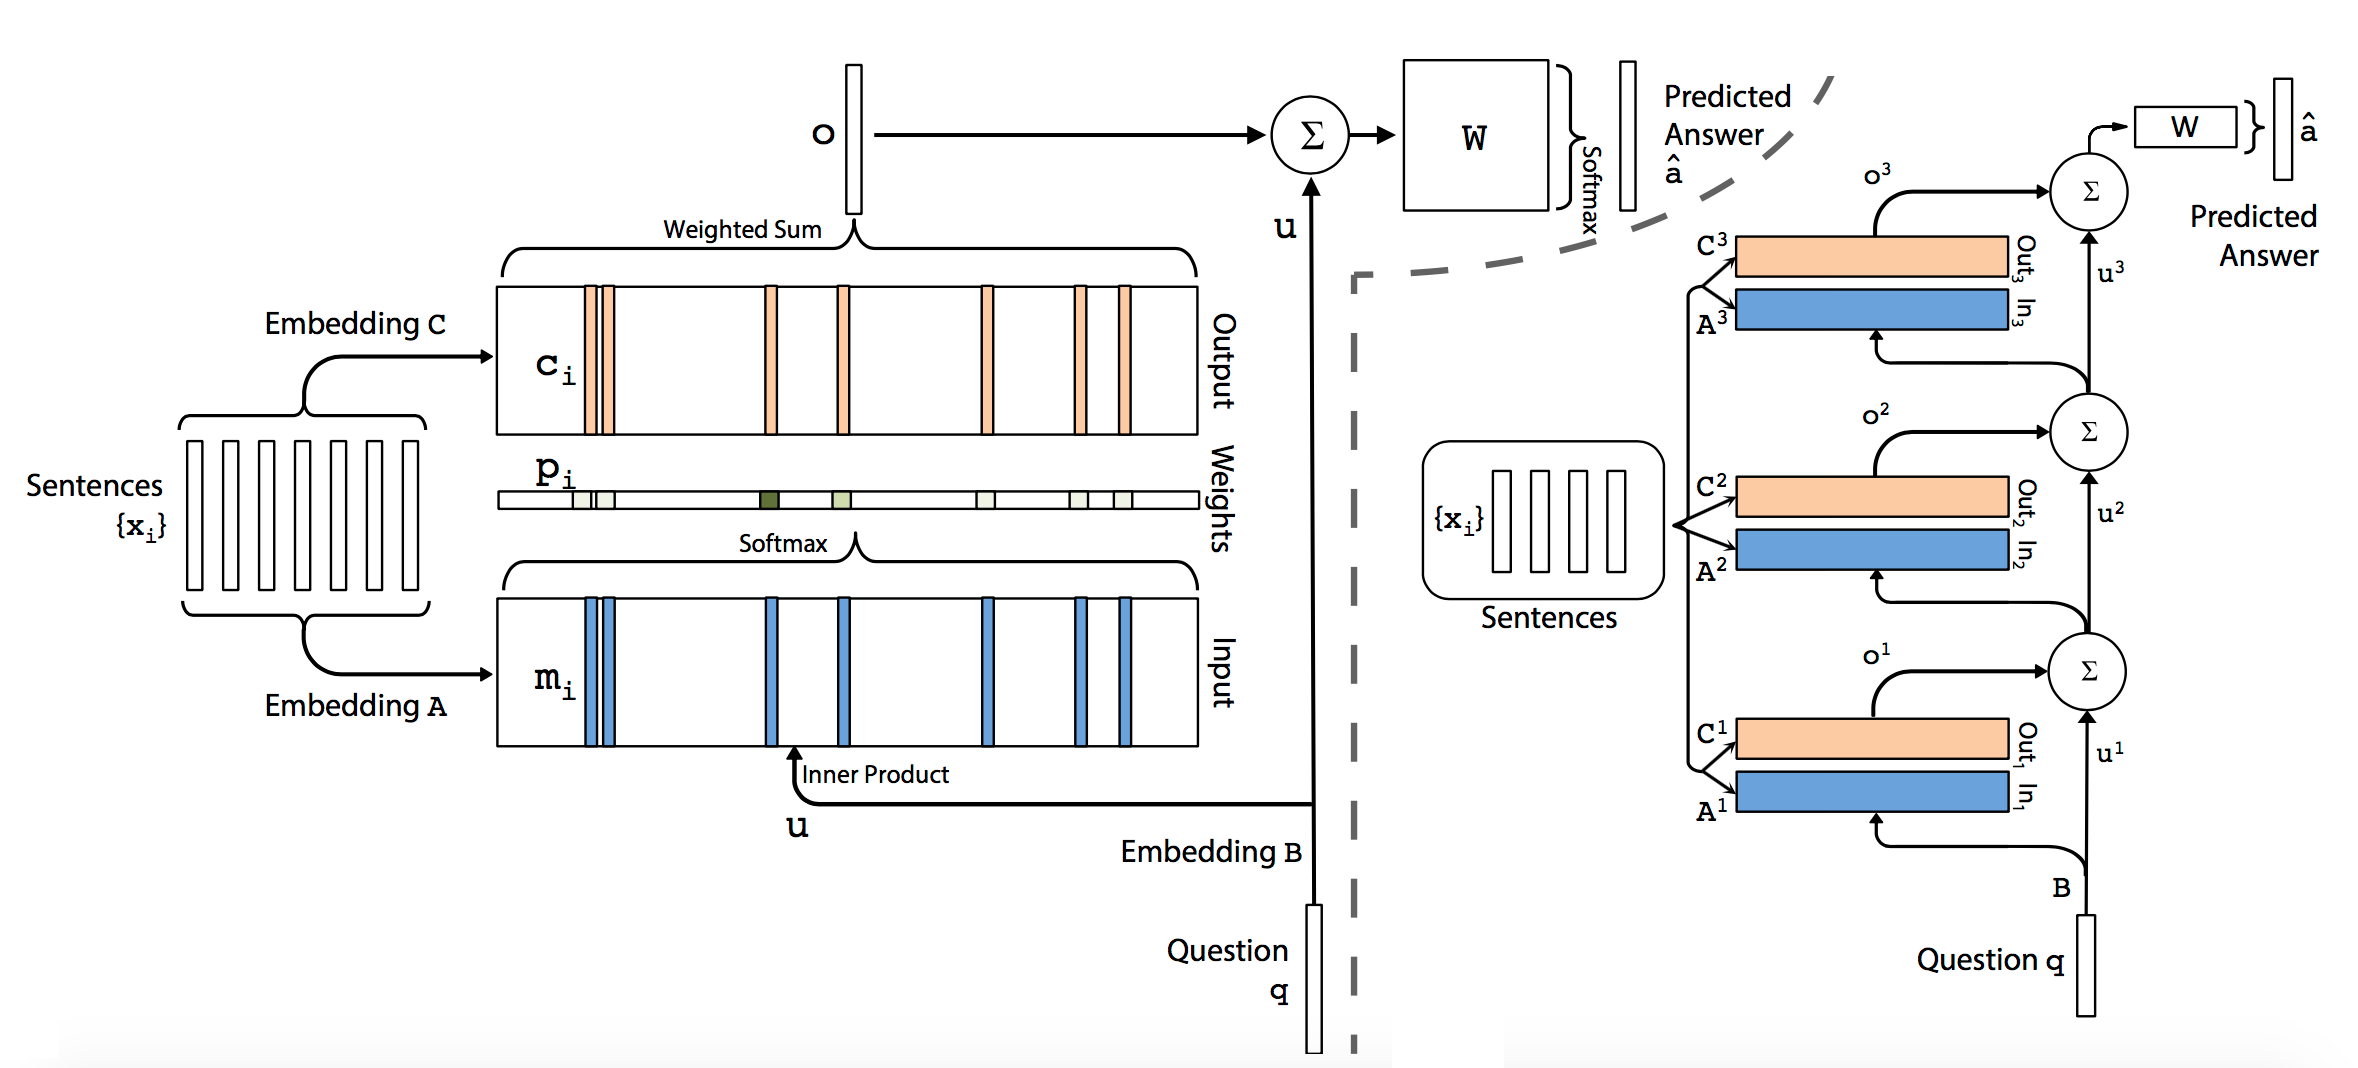
\includegraphics[width=0.7\textwidth]{mem.png}
    \caption{1-Hop and 3-Hop  MeMNetwork}
\end{center}
\end{figure}

\noindent But as one can see on figure 1, we can in fact stack mutliple hops to memory, in this case 3. This would increase performance when dealing with tasks that would require reasoning on more than one fact. In more details, we define the intermediate outputs $o_k$ and $u_k$ by:
\begin{gather*}
o_k  = \sum\limits_{i=1}softmax(u_k^Tm_i) \\
u_{k+1}  = u_k + o_k
\end{gather*} 

\subsection{Parameters Tying}
As mentioned in \cite{mem}, if using multiple hops to memory yields better results, it also has for consequence to increase significantly the number of parameters. We therefore investigated two different constraints on the embedding matrics $A_i$ and $C_i$, known as parameter tying:
\begin{itemize}
\item \textbf{Adjacent}: $A_{i+1} = C_i$ i.e. the current output embedding is equal to the next input embedding,
\item \textbf{Layer-wise or RNN-like}:  $A_{i+1} = A_i$ and  $C_{i+1} = C_i$ for all $i$
\end{itemize}
When using the RNN-like tying, it is prefered to use define $u_{i+1}$ as a linear transformation of $u_k$, i.e. $u_{i+1} = H u_{i} + o_{i}$. We will compare results using the two different tying methods in the next section.

\section{Experiment}
\subsection{Data and Preprocessing}

Our goal is to build a robust model, i.e. working on any kind of tasks of question answering. The bAbI dataset created by Facebook \cite{aiqua} provides us relevant tasks. We pre-processed it with several steps.

First, we mapped each word to an index. We know that every answer word from the test set is used as anwser in the train set, so this index is built only on the train set but used for both train and test set.

Second, we pre-process each sentence as a bag-of-words, i.e. we convert it to a vector of word indexes of fixed length (the maximum length over the sentences), using a padding index of 0 at the end. We separate in two different arrays the sentences and the questions, both are indexed globally in the given dataset.

Third, we encoded in one array the links between the questions and the sentences. Each row corresponds to the question with the corresponding global index in the dataset and contains: index of the first and last sentences of the story and the indexes of its supporting facts. This later is a fixed size list, with a 0 padding for question with less supporting facts. However, our models are weakly supervised so we don't use these supporting facts as we aim to build a robust model that we could apply on any QA tasks.

Finally, we store in one vector the word index of the answer for each question. In the case of an answer containing multiple words, we extend the vocabulary with this sequence of words as a new word. 

\subsection{Implementation Details}

\noindent We tested multiple hacks in order to improve performance that we will now detail.

\paragraph{Temporal Encoding}
In order to account for a certain notion of temporality in our baseline model, we weighted word occurences differently based on how close these words were from the question. For the memory network, we add to both the input and output memories, temporal matrices $T_{A_i}$ and $T_{C_i}$ that will be learn during training, and to which we apply the same parameter constraints as $A_i$ and $C_i$. We refer to Temporal Encoding as TE.
 
\paragraph{Position Encoding}
We choose to represent sentence embeddings as the sum of its words' embeddings for simplicity reasons. Indeed, it was then possible to obtain a standard size of each entry in the memory, equal to the hidden embedding size. Nevertheless, this choice could potentially loose information about word position that concatenation would pick up. To avoid this loss of information, we replace the current memory representation:$$m_i = \sum_j Ax_{ij}$$ by $$m_i = \sum_j l_j\cdot A x_{ij}$$ where $\cdot$ corresponds to the element-wise multiplication and $l_j$ is a fixed vector with entries defined by: $$l_kj = (1-\frac{j}{J})-\frac{k}{D}(1-2\frac{j}{J})$$ with $j$ being the indexed of the sentence, $J$ the number of sentences allowed in memory and $D$ the hidden dimension of embeddings. We refer to position encoding as PE.

\paragraph{Stochastic Gradient Descent}
We used a stochastic gradient descent to fit the parameters of the different layers. In the multiple hops architecture as the backpropagation is quite long, we constrained the $l_2$ norm of the gradient to be below 40 (we set it to 40 when larger). We also annealed the learning rate $eta$ every 15 epochs to refine the training over the epochs.

\subsection{Results}

In order to compare our results with the ones from \cite{mem}, we decided to adopt the same hyperparameters, i.e.:
\begin{itemize}
\item Capped the memory at 50 sentences,
\item Used an embedding dimension equal to: $d=50$,
\item Train using 100 epochs,
\item Used a learning rate of 0.01 which was halfed every 20 iterations.
\end{itemize}
\noindent We did not use batching (even if we implemented it) because of a rather fast training time. Finally, switching to a GPU took more training time due to a poor level of paralisation.\\

\noindent We now summarise the results of our experiments in the following tables:

\begin{table}[H]
\centering
\label{my-label}
 \resizebox{1\textwidth}{6cm}{
\begin{tabular}{ccccccccclcc}
\multicolumn{1}{l}{}                                                                              & \multicolumn{1}{l}{}                                                                & \multicolumn{1}{l}{}                                                                           &                                                                                          & \cellcolor[HTML]{FFCCC9}Best                                                             & \cellcolor[HTML]{ECF4FF}Second Best                                                      &                                                                                             & \cellcolor[HTML]{67FD9A}\begin{tabular}[c]{@{}c@{}}Inexplicable\\ Difference\end{tabular}   &                                                                                             &                                          &                                                                                                &                                                                                                \\
\multicolumn{1}{l}{}                                                                              & \multicolumn{1}{l}{}                                                                & \multicolumn{1}{l}{}                                                                           & \multicolumn{1}{l}{}                                                                     & \multicolumn{1}{l}{}                                                                     & \multicolumn{1}{l}{}                                                                     & \multicolumn{1}{l}{}                                                                        & \multicolumn{1}{l}{}                                                                        &                                                                                             &                                          & \multicolumn{1}{l}{}                                                                           & \multicolumn{1}{l}{}                                                                           \\ \cline{3-9} \cline{11-12} 
\multicolumn{1}{l}{}                                                                              & \multicolumn{1}{l|}{}                                                               & \multicolumn{6}{c|}{Jointly Trained}                                                                                                                                                                                                                                                                                                                                                                                                                                                                                                                                        & \multicolumn{1}{c|}{Individually trained}                                                   & \multicolumn{1}{l|}{}                    & \multicolumn{2}{c|}{\begin{tabular}[c]{@{}c@{}}Sukhbaatar et al\\ Jointly Trained\end{tabular}}                                                                                                 \\ \hline
\multicolumn{1}{|c|}{Task}                                                                        & \multicolumn{1}{c|}{\begin{tabular}[c]{@{}c@{}}Count-Based\\ Baseline\end{tabular}} & \multicolumn{1}{c|}{\begin{tabular}[c]{@{}c@{}}3-hop MemNN\\ RNN-Like\\ TE  + PE\end{tabular}} & \multicolumn{1}{c|}{\begin{tabular}[c]{@{}c@{}}1-hop MemNN\\ Adjacent\\ TE\end{tabular}} & \multicolumn{1}{c|}{\begin{tabular}[c]{@{}c@{}}2-hop MemNN\\ Adjacent\\ TE\end{tabular}} & \multicolumn{1}{c|}{\begin{tabular}[c]{@{}c@{}}3-hop MemNN\\ Adjacent\\ TE\end{tabular}} & \multicolumn{1}{c|}{\begin{tabular}[c]{@{}c@{}}2-hop MemNN\\ Adjacent\\ TE+PE\end{tabular}} & \multicolumn{1}{c|}{\begin{tabular}[c]{@{}c@{}}3-hop MemNN\\ Adjacent\\ TE+PE\end{tabular}} & \multicolumn{1}{c|}{\begin{tabular}[c]{@{}c@{}}3-hop MemNN\\ Adjacent\\ TE+PE\end{tabular}} & \multicolumn{1}{l|}{}                    & \multicolumn{1}{c|}{\begin{tabular}[c]{@{}c@{}}3-hop MemNN\\ Adjacent\\ TE+PE+LS\end{tabular}} & \multicolumn{1}{c|}{\begin{tabular}[c]{@{}c@{}}3-hop MemNN\\ RNN-Like\\ TE+PE+LS\end{tabular}} \\ \cline{1-9} \cline{11-12} 
\multicolumn{1}{|c|}{1}                                                                           & \multicolumn{1}{c|}{0.5}                                                            & \multicolumn{1}{c|}{0.99}                                                                      & \multicolumn{1}{c|}{\cellcolor[HTML]{FFCCC9}{\color[HTML]{333333} 1}}                    & \multicolumn{1}{c|}{0.97}                                                                & \multicolumn{1}{c|}{\cellcolor[HTML]{ECF4FF}0.99}                                        & \multicolumn{1}{c|}{\cellcolor[HTML]{FFCCC9}1}                                              & \multicolumn{1}{c|}{\cellcolor[HTML]{ECF4FF}0.99}                                           & \multicolumn{1}{c|}{\cellcolor[HTML]{FFCCC9}1}                                              & \multicolumn{1}{l|}{}                    & \multicolumn{1}{c|}{0.99}                                                                      & \multicolumn{1}{c|}{0.99}                                                                      \\ \cline{1-1}
\multicolumn{1}{|c|}{2}                                                                           & \multicolumn{1}{c|}{0.4}                                                            & \multicolumn{1}{c|}{\cellcolor[HTML]{ECF4FF}0.79}                                              & \multicolumn{1}{c|}{0.24}                                                                & \multicolumn{1}{c|}{0.25}                                                                & \multicolumn{1}{c|}{0.37}                                                                & \multicolumn{1}{c|}{\cellcolor[HTML]{FFCCC9}0.88}                                           & \multicolumn{1}{c|}{\cellcolor[HTML]{FFFFFF}0.78}                                           & \multicolumn{1}{c|}{0.31}                                                                   & \multicolumn{1}{l|}{}                    & \multicolumn{1}{c|}{0.86}                                                                      & \multicolumn{1}{c|}{0.81}                                                                      \\ \cline{1-1}
\multicolumn{1}{|c|}{3}                                                                           & \multicolumn{1}{c|}{0.26}                                                           & \multicolumn{1}{c|}{0.36}                                                                      & \multicolumn{1}{c|}{0.21}                                                                & \multicolumn{1}{c|}{0.25}                                                                & \multicolumn{1}{c|}{0.21}                                                                & \multicolumn{1}{c|}{\cellcolor[HTML]{ECF4FF}0.65}                                           & \multicolumn{1}{c|}{\cellcolor[HTML]{FFCCC9}0.676}                                          & \multicolumn{1}{c|}{0.33}                                                                   & \multicolumn{1}{l|}{}                    & \multicolumn{1}{c|}{0.76}                                                                      & \multicolumn{1}{c|}{0.68}                                                                      \\ \cline{1-1}
\multicolumn{1}{|c|}{4}                                                                           & \multicolumn{1}{c|}{0.34}                                                           & \multicolumn{1}{c|}{\cellcolor[HTML]{FFCCC9}0.86}                                              & \multicolumn{1}{c|}{0.66}                                                                & \multicolumn{1}{c|}{0.65}                                                                & \multicolumn{1}{c|}{0.66}                                                                & \multicolumn{1}{c|}{0.77}                                                                   & \multicolumn{1}{c|}{\cellcolor[HTML]{ECF4FF}0.81}                                           & \multicolumn{1}{c|}{0.81}                                                                   & \multicolumn{1}{l|}{}                    & \multicolumn{1}{c|}{0.94}                                                                      & \multicolumn{1}{c|}{0.83}                                                                      \\ \cline{1-1}
\multicolumn{1}{|c|}{5}                                                                           & \multicolumn{1}{c|}{0.48}                                                           & \multicolumn{1}{c|}{\cellcolor[HTML]{ECF4FF}0.84}                                              & \multicolumn{1}{c|}{0.83}                                                                & \multicolumn{1}{c|}{0.82}                                                                & \multicolumn{1}{c|}{0.83}                                                                & \multicolumn{1}{c|}{\cellcolor[HTML]{ECF4FF}0.84}                                           & \multicolumn{1}{c|}{\cellcolor[HTML]{FFCCC9}0.96}                                           & \multicolumn{1}{c|}{\cellcolor[HTML]{ECF4FF}0.84}                                           & \multicolumn{1}{l|}{}                    & \multicolumn{1}{c|}{0.85}                                                                      & \multicolumn{1}{c|}{0.87}                                                                      \\ \cline{1-1}
\multicolumn{1}{|c|}{6}                                                                           & \multicolumn{1}{c|}{0.5}                                                            & \multicolumn{1}{c|}{\cellcolor[HTML]{ECF4FF}0.97}                                              & \multicolumn{1}{c|}{0.76}                                                                & \multicolumn{1}{c|}{0.93}                                                                & \multicolumn{1}{c|}{0.93}                                                                & \multicolumn{1}{c|}{\cellcolor[HTML]{FFCCC9}0.99}                                           & \multicolumn{1}{c|}{0.83}                                                                   & \multicolumn{1}{c|}{0.92}                                                                   & \multicolumn{1}{l|}{}                    & \multicolumn{1}{c|}{0.97}                                                                      & \multicolumn{1}{c|}{0.98}                                                                      \\ \cline{1-1}
\multicolumn{1}{|c|}{7}                                                                           & \multicolumn{1}{c|}{0.49}                                                           & \multicolumn{1}{c|}{0.85}                                                                      & \multicolumn{1}{c|}{0.84}                                                                & \multicolumn{1}{c|}{0.82}                                                                & \multicolumn{1}{c|}{0.86}                                                                & \multicolumn{1}{c|}{\cellcolor[HTML]{ECF4FF}0.87}                                           & \multicolumn{1}{c|}{\cellcolor[HTML]{FFCCC9}0.89}                                           & \multicolumn{1}{c|}{0.79}                                                                   & \multicolumn{1}{l|}{}                    & \multicolumn{1}{c|}{0.82}                                                                      & \multicolumn{1}{c|}{0.90}                                                                      \\ \cline{1-1}
\multicolumn{1}{|c|}{8}                                                                           & \multicolumn{1}{c|}{0.28}                                                              & \multicolumn{1}{c|}{\cellcolor[HTML]{ECF4FF}0.90}                                              & \multicolumn{1}{c|}{0.89}                                                                & \multicolumn{1}{c|}{0.87}                                                                & \multicolumn{1}{c|}{\cellcolor[HTML]{ECF4FF}0.90}                                        & \multicolumn{1}{c|}{\cellcolor[HTML]{ECF4FF}0.90}                                           & \multicolumn{1}{c|}{\cellcolor[HTML]{FFCCC9}0.98}                                           & \multicolumn{1}{c|}{0.88}                                                                   & \multicolumn{1}{l|}{}                    & \multicolumn{1}{c|}{0.90}                                                                      & \multicolumn{1}{c|}{0.94}                                                                      \\ \cline{1-1}
\multicolumn{1}{|c|}{9}                                                                           & \multicolumn{1}{c|}{0.64}                                                           & \multicolumn{1}{c|}{0.95}                                                                      & \multicolumn{1}{c|}{0.80}                                                                & \multicolumn{1}{c|}{\cellcolor[HTML]{ECF4FF}0.96}                                        & \multicolumn{1}{c|}{0.95}                                                                & \multicolumn{1}{c|}{\cellcolor[HTML]{FFCCC9}0.99}                                           & \multicolumn{1}{c|}{0.94}                                                                   & \multicolumn{1}{c|}{0.76}                                                                   & \multicolumn{1}{l|}{}                    & \multicolumn{1}{c|}{0.97}                                                                      & \multicolumn{1}{c|}{0.99}                                                                      \\ \cline{1-1}
\multicolumn{1}{|c|}{10}                                                                          & \multicolumn{1}{c|}{0.44}                                                           & \multicolumn{1}{c|}{0.81}                                                                      & \multicolumn{1}{c|}{0.68}                                                                & \multicolumn{1}{c|}{\cellcolor[HTML]{ECF4FF}0.90}                                        & \multicolumn{1}{c|}{0.87}                                                                & \multicolumn{1}{c|}{\cellcolor[HTML]{FFCCC9}0.95}                                           & \multicolumn{1}{c|}{\cellcolor[HTML]{ECF4FF}0.90}                                           & \multicolumn{1}{c|}{0.66}                                                                   & \multicolumn{1}{l|}{}                    & \multicolumn{1}{c|}{0.94}                                                                      & \multicolumn{1}{c|}{0.97}                                                                      \\ \cline{1-1}
\multicolumn{1}{|c|}{11}                                                                          & \multicolumn{1}{c|}{0.63}                                                           & \multicolumn{1}{c|}{\cellcolor[HTML]{ECF4FF}0.95}                                              & \multicolumn{1}{c|}{0.91}                                                                & \multicolumn{1}{c|}{0.90}                                                                & \multicolumn{1}{c|}{0.91}                                                                & \multicolumn{1}{c|}{\cellcolor[HTML]{FFCCC9}0.97}                                           & \multicolumn{1}{c|}{0.93}                                                                   & \multicolumn{1}{c|}{0.86}                                                                   & \multicolumn{1}{l|}{}                    & \multicolumn{1}{c|}{0.99}                                                                      & \multicolumn{1}{c|}{0.97}                                                                      \\ \cline{1-1}
\multicolumn{1}{|c|}{12}                                                                          & \multicolumn{1}{c|}{0.60}                                                           & \multicolumn{1}{c|}{\cellcolor[HTML]{ECF4FF}0.99}                                              & \multicolumn{1}{c|}{1}                                                                   & \multicolumn{1}{c|}{0.97}                                                                & \multicolumn{1}{c|}{\cellcolor[HTML]{FFCCC9}1}                                           & \multicolumn{1}{c|}{\cellcolor[HTML]{FFCCC9}1}                                              & \multicolumn{1}{c|}{0.93}                                                                   & \multicolumn{1}{c|}{\cellcolor[HTML]{FFCCC9}1}                                              & \multicolumn{1}{l|}{}                    & \multicolumn{1}{c|}{0.99}                                                                      & \multicolumn{1}{c|}{1}                                                                         \\ \cline{1-1}
\multicolumn{1}{|c|}{13}                                                                          & \multicolumn{1}{c|}{0.68}                                                           & \multicolumn{1}{c|}{\cellcolor[HTML]{FFCCC9}0.99}                                              & \multicolumn{1}{c|}{\cellcolor[HTML]{ECF4FF}0.94}                                        & \multicolumn{1}{c|}{0.87}                                                                & \multicolumn{1}{c|}{\cellcolor[HTML]{ECF4FF}0.94}                                        & \multicolumn{1}{c|}{\cellcolor[HTML]{FFCCC9}0.99}                                           & \multicolumn{1}{c|}{0.93}                                                                   & \multicolumn{1}{c|}{0.92}                                                                   & \multicolumn{1}{l|}{}                    & \multicolumn{1}{c|}{0.98}                                                                      & \multicolumn{1}{c|}{0.99}                                                                      \\ \cline{1-1}
\multicolumn{1}{|c|}{14}                                                                          & \multicolumn{1}{c|}{0.29}                                                           & \multicolumn{1}{c|}{0.79}                                                                      & \multicolumn{1}{c|}{0.65}                                                                & \multicolumn{1}{c|}{\cellcolor[HTML]{FFCCC9}0.94}                                        & \multicolumn{1}{c|}{0.84}                                                                & \multicolumn{1}{c|}{\cellcolor[HTML]{FFCCC9}0.94}                                           & \multicolumn{1}{c|}{0.84}                                                                   & \multicolumn{1}{c|}{\cellcolor[HTML]{ECF4FF}0.87}                                           & \multicolumn{1}{l|}{}                    & \multicolumn{1}{c|}{0.92}                                                                      & \multicolumn{1}{c|}{0.98}                                                                      \\ \cline{1-1}
\multicolumn{1}{|c|}{15}                                                                          & \multicolumn{1}{c|}{0.14}                                                           & \multicolumn{1}{c|}{\cellcolor[HTML]{FFCCC9}0.55}                                              & \multicolumn{1}{c|}{0.41}                                                                & \multicolumn{1}{c|}{0.33}                                                                & \multicolumn{1}{c|}{0.40}                                                                & \multicolumn{1}{c|}{0.38}                                                                   & \multicolumn{1}{c|}{0.42}                                                                   & \multicolumn{1}{c|}{\cellcolor[HTML]{ECF4FF}0.50}                                           & \multicolumn{1}{l|}{}                    & \multicolumn{1}{c|}{\cellcolor[HTML]{67FD9A}1}                                                 & \multicolumn{1}{c|}{0.98}                                                                      \\ \cline{1-1}
\multicolumn{1}{|c|}{16}                                                                          & \multicolumn{1}{c|}{0.52}                                                           & \multicolumn{1}{c|}{\cellcolor[HTML]{ECF4FF}0.50}                                              & \multicolumn{1}{c|}{\cellcolor[HTML]{FFCCC9}0.51}                                        & \multicolumn{1}{c|}{0.47}                                                                & \multicolumn{1}{c|}{0.49}                                                                & \multicolumn{1}{c|}{0.49}                                                                   & \multicolumn{1}{c|}{0.45}                                                                   & \multicolumn{1}{c|}{0.49}                                                                   & \multicolumn{1}{l|}{}                    & \multicolumn{1}{c|}{\cellcolor[HTML]{67FD9A}0.96}                                              & \multicolumn{1}{c|}{0.49}                                                                      \\ \cline{1-1}
\multicolumn{1}{|c|}{17}                                                                          & \multicolumn{1}{c|}{0.48}                                                           & \multicolumn{1}{c|}{0.56}                                                                      & \multicolumn{1}{c|}{0.49}                                                                & \multicolumn{1}{c|}{0.52}                                                                & \multicolumn{1}{c|}{\cellcolor[HTML]{FFCCC9}0.59}                                        & \multicolumn{1}{c|}{0.55}                                                                   & \multicolumn{1}{c|}{0.54}                                                                   & \multicolumn{1}{c|}{\cellcolor[HTML]{ECF4FF}0.57}                                           & \multicolumn{1}{l|}{}                    & \multicolumn{1}{c|}{0.56}                                                                      & \multicolumn{1}{c|}{0.58}                                                                      \\ \cline{1-1}
\multicolumn{1}{|c|}{18}                                                                          & \multicolumn{1}{c|}{0.53}                                                           & \multicolumn{1}{c|}{0.79}                                                                      & \multicolumn{1}{c|}{0.48}                                                                & \multicolumn{1}{c|}{0.49}                                                                & \multicolumn{1}{c|}{0.47}                                                                & \multicolumn{1}{c|}{0.55}                                                                   & \multicolumn{1}{c|}{\cellcolor[HTML]{ECF4FF}0.90}                                           & \multicolumn{1}{c|}{\cellcolor[HTML]{FFCCC9}0.92}                                           & \multicolumn{1}{l|}{}                    & \multicolumn{1}{c|}{0.90}                                                                      & \multicolumn{1}{c|}{0.91}                                                                      \\ \cline{1-1}
\multicolumn{1}{|c|}{19}                                                                          & \multicolumn{1}{c|}{0}                                                              & \multicolumn{1}{c|}{0.01}                                                                      & \multicolumn{1}{c|}{0.09}                                                                & \multicolumn{1}{c|}{0.08}                                                                & \multicolumn{1}{c|}{0.11}                                                                & \multicolumn{1}{c|}{\cellcolor[HTML]{ECF4FF}0.13}                                           & \multicolumn{1}{c|}{\cellcolor[HTML]{FFCCC9}0.18}                                           & \multicolumn{1}{c|}{0.11}                                                                   & \multicolumn{1}{l|}{}                    & \multicolumn{1}{c|}{0.1}                                                                       & \multicolumn{1}{c|}{0.09}                                                                      \\ \cline{1-1}
\multicolumn{1}{|c|}{20}                                                                          & \multicolumn{1}{c|}{0.52}                                                           & \multicolumn{1}{c|}{\cellcolor[HTML]{FFCCC9}0.97}                                              & \multicolumn{1}{c|}{0.92}                                                                & \multicolumn{1}{c|}{0.92}                                                                & \multicolumn{1}{c|}{0.92}                                                                & \multicolumn{1}{c|}{\cellcolor[HTML]{ECF4FF}0.95}                                           & \multicolumn{1}{c|}{0.92}                                                                   & \multicolumn{1}{c|}{0.92}                                                                   & \multicolumn{1}{l|}{}                    & \multicolumn{1}{c|}{1}                                                                         & \multicolumn{1}{c|}{0.99}                                                                      \\ \cline{1-9} \cline{11-12} 
\multicolumn{1}{|c|}{TOTAL}                                                                       & \multicolumn{1}{c|}{0.44}                                                           & \multicolumn{1}{c|}{0.77}                                                                      & \multicolumn{1}{c|}{0.67}                                                                & \multicolumn{1}{c|}{0.69}                                                                & \multicolumn{1}{c|}{0.71}                                                                & \multicolumn{1}{c|}{\cellcolor[HTML]{FFCCC9}0.79}                                           & \multicolumn{1}{c|}{\cellcolor[HTML]{ECF4FF}0.78}                                           & \multicolumn{1}{c|}{0.72}                                                                   & \multicolumn{1}{l|}{}                    & \multicolumn{1}{c|}{0.87}                                                                      & \multicolumn{1}{c|}{0.85}                                                                      \\ \cline{1-9} \cline{11-12} 
\multicolumn{1}{|c|}{\begin{tabular}[c]{@{}c@{}}Failed Tasks\\ (Acc \textless 0.95)\end{tabular}} & \multicolumn{1}{c|}{20}                                                             & \multicolumn{1}{c|}{13}                                                                        & \multicolumn{1}{c|}{20}                                                                  & \multicolumn{1}{c|}{17}                                                                  & \multicolumn{1}{c|}{17}                                                                  & \multicolumn{1}{c|}{12}                                                                     & \multicolumn{1}{c|}{17}                                                                     & \multicolumn{1}{c|}{18}                                                                     & \multicolumn{1}{l|}{\multirow{-23}{*}{}} & \multicolumn{1}{c|}{11}                                                                        & \multicolumn{1}{c|}{10}                                                                        \\ \cline{1-9} \cline{11-12} 
\end{tabular}
}
\caption{Accuracy Results on held-out test data}
\end{table}
\noindent We would first like to note that we experienced quite a lot of variance with the results of the memory networks. We therefore had to train the models several times and showed above the best results. \\

\noindent The first obvious result from this table is the signaficant difference between our count based baseline and the memory networks. Nevertheless, we were quite surprise to get an accuracy for our baseline that surpasses the one in the original paper by Weston et al. presenting the bAbi datatest (424\% vs 34\%). The second observation we can make is that performing multiple hops to memory increases accuracy but also the number of succesful tasks (i.e. tasks where accuracy is above 95\%). Based on our experiments, it is however not the case that the more hops to memory, the better the accuracy. If all results shown in this table were obtained using temporal encoding, experimenting with and without showed significant improvent with it, as well as with position encoding. What is interesting to note is that the global performance is relatively good, as most the tasks have a scores above 80\% and only a few task failed completely with scores around or below 50\%. Agent's motivation (task 20) remains the only task where the model absolutely fails (with scores close to 0). 

\noindent Finally, comparing our results with the ones form Sukhbaatar et al, we can see that we are not very far form their results. Nevertheless, our average accuracy was negatively impacted by significant differences on two tasks (basic deduction and induction) which were highlighted in green. We also observed that adjacent tying worked on average better than RNN-like tying and training all tasks together yielded better results, even if some tasks trained individually would work slightly better.

\section{Future Work}
\subsection{Application to the MCTest dataset}
Results on the bAbi dataset were encouraging but have to be put in perspective. Indeed, the size and quality of the stories, the number of words in the vocabulary, the fact that answers appear both in the training and test data make it a rather easy dataset to work on. In order to challenge the algorithm, we wanted to test it on the MCTest dataset \cite{mctest}. This dataset contains 660 stories and multiple choice questions with sentences answers. For instance:
\begin{framed}
\begin{center}
Q:  What did James do after he ordered the fries?\\
A) went to the grocery store\\
B) went home without paying\\
C) ate them\\
D) made up his mind to be a better turle\\
\end{center}
\end{framed}
\noindent With these types of question, we can not use the same trick as for the bAby, i.e. use a final linear model and softmax layer to predict a distribution over possible answers that appeared in the training set. What we propose instead is to introduce a matrix $D$ used to embed the answers and store them in $a_1, a_2, a_3$ and $a_4$ and use the last intermediate output $u_K = u_{K-1} + o_{K-1}$ (where $K$ is the number of hops) to evaluate the cosine similarity with the $a_i$'s:
$$sim(u_K,a_i) = \frac{u_K \cdot a_i}{||u_K||\,||a_i||}.$$ We can then normalise the scores using a softmax transformation and use regular NNL loss to train the model.

\subsection{Dynamic Memory Networks}

The work from \cite{dmn} suggests two major extensions for our work. 

\paragraph*{Encoding}
First, we encodes both the input and question as a (weighted in case of the position encoding) sum of the embeddings of the words of each sentence. This produces for the question a single vector in the hidden space and for the input we have as many vectors as space in our memory. Instead, we could encode a given sentence (either the question or a sentence of the input) with a recurrent architecture. We feed this architecture sequentially with the different words to update the hidden state and the sentence representation would be the last hidden state (i.e. the one output on the end-of-sentence token).
\cite{dmn} suggests to use a Gated Recurrent Unit \cite{gru} as recurrent architecture as it provides promising results. More formarly, for a given story, we extract the bag-of-words for the whole story with the insertion of an end-of-sentence token between each sentence. We feed this bag-of-words to the encoder network and update its hidden state as follows at the timesteps $t$ (i.e. the $t^{th}$ word of the bow) : $h_t = GRU(L[x_t], h_{t-1})$, with $L$ the embedding matrix. The new encoding of the whole story of $S$ sentences will be the sequence of the hidden states at each end-of-sentence token. We encode similarly the question in one vector corresponding to the hidden state after the last word.

\paragraph*{Episodic Memory}

A more advanced extension would be to apply their extension which enables to update the memory based on episodes computed with both an attention mechanism and a recurrent network. The architecture is well detailed in \citep{dmn}. This could improve our approach in combining the different inputs into memory facts. We do this combination with a multiple hops approach where we update our memory at each hop based on the current combined representation of the question and the supporting memory. This alternative method could build a more advanced memory.

\section{Conclusion}

This project gave us the opportunity to build our own end-to-end memory network and to apply it on a well known dataset for non-factoid question answering. We realized how useful the memory component is to solve these tasks in comparison to a simple count based approach. However, the model still underperforms some tasks and extensions can still be considered, for instance to use a dynamic memory. Another extension will be to test this architecture on a multiple choice questions as provided in \cite{mctest}

\section{Acknowledgement}

We would like to thank the staff from CS 287 Statistical Natural Language Processing for their advice and for providing this great course. In particular, we are thankful towards the professor Alexander "Sasha" Rush and the TAs Sam Wiseman and Saketh Rama.

\vskip 0.2in
\bibliography{sample}

\section{Appendix}
\begin{table}[H]
\centering
\label{my-label}
\begin{tabular}{c|c}
Task number & Description          \\ \hline \hline
1           & 1 supporting fact    \\
2           & 2 supporting facts   \\
3           & 3 supporting facts   \\
4           & 2 argument relations \\
5           & 3 argument relations \\
6           & yes/no               \\
7           & counting             \\
8           & list/set             \\
9           & simple negation      \\
10          & indefinite knowledge \\
11          & basic coreference    \\
12          & conjunction          \\
13          & compound coreference \\
14          & time reasoning       \\
15          & basic deduction      \\
16          & basic induction      \\
17          & positional reasoning \\
18          & size reasoning       \\
19          & path finding         \\
20          & agent's motivation  
\end{tabular}
\caption{Appendix 1: Description of tasks}
\end{table}

\end{document}